\documentclass{beamer}
%
% Choose how your presentation looks.
%
% For more themes, color themes and font themes, see:
% http://deic.uab.es/~iblanes/beamer_gallery/index_by_theme.html
%
\mode<presentation>
{
  \usetheme{Darmstadt}      % or try Darmstadt, Madrid, Warsaw, ...
  \usecolortheme{crane} % or try albatross, beaver, crane, ...
  \usefonttheme{default}  % or try serif, structurebold, ...
  \setbeamertemplate{navigation symbols}{}
  \setbeamertemplate{caption}[numbered]
  \usepackage{tikz}
  \usepackage{pgfplots}
  \usepackage{pgf}
  \usepackage{units}
  \usepackage{metalogo}
  \usepackage{graphicx}
  \usepackage{caption}
  \usepackage{subcaption}
  \usepackage[mode=buildnew]{standalone}% requires -shell-escape
  \usepgfplotslibrary{groupplots}
  \usepackage{amsmath}
} 

\usepackage[english]{babel}
\usepackage[utf8x]{inputenc}
\setbeamertemplate{footline}[frame number]

\title{LAS Thesis project kickoff meeting}
\author{Moritz Wolter}

\date{\today}

\begin{document}
\begin{frame}
  \titlepage
\end{frame}


% Uncomment these lines for an automatically generated outline.
\begin{frame}{Outline}
  \tableofcontents
\end{frame}

\section{Project Overview}
\begin{frame}{Project Overview}
	\begin{itemize}
		\item Transcribe speech utterances to characters. 
		\item Use a listen attend and spell (LAS) model to do this.
		\item Train model components jointly.
	\end{itemize}
\end{frame}

\section{Listen Attend and Spell}

\begin{frame}{The LAS-Architecture}
	\begin{figure}
		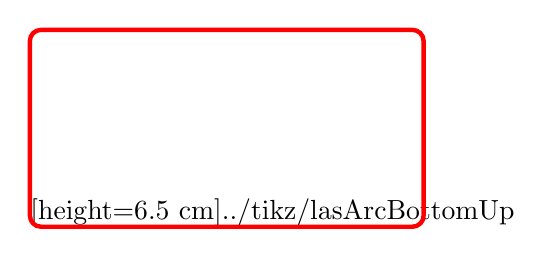
\begin{tikzpicture}
		    \node[anchor=south west,inner sep=0] at (0,0) {\includestandalone[height=6.5 cm]{../tikz/lasArcBottomUp}};
		    \draw[red,ultra thick,rounded corners] (0.0,0.0) rectangle (5.0,2.5);
		\end{tikzpicture}
		\caption{The LAS architecture}
		\label{fig:las}
	\end{figure}
\end{frame}

\begin{frame}{Debugging The Listener}
	\begin{figure}
		\includestandalone[height=6.5 cm]{../tikz/blstmCTC}
		\caption{BLSTM CTC schematic}
	\end{figure}
\end{frame}


\begin{frame}{First Results on Timit}
	\begin{figure}
		\includestandalone[height=6.5 cm]{../tikz/ctc2LayerBLSTMclippedGrad}
		\caption{BLSTM-CTC training and validation error on timit.}
	\end{figure}
\end{frame}


\section{Planning}
\begin{frame}{What happend so far? What will happen next?}
\begin{itemize}
\item What happend so far?
	\begin{enumerate}
		\item Listener with CTC on Timit .
	\end{enumerate}
\item What will happen next?
		\begin{enumerate}
			\item Switch to Aurora4.
			\item Test the CTC-listener on Aurora4. 
			\item Add attention based spelling to the listener.
			\item Decoding with beam search.
		\end{enumerate}
\item After that you take over!		
	 \begin{enumerate}
	 	\item Test the las skeleton on LibriSpeech.
	 \end{enumerate}
\end{itemize}
\end{frame}


\section{Questions}
\begin{frame}{Questions}
	Thank you for your attention. Questions? \\
	\texttt{moritzalexander.wolter@student.kuleuven.be} \\
	or come and meet me in our LAS-room (02.88).
\end{frame}


\end{document}
